% AEJ-Article.tex for AEA last revised 22 June 2011
\documentclass[PP]{AEA}

%%%%%% NOTE FROM OVERLEAF: The mathtime package is no longer publicly available nor distributed. We recommend using a different font package e.g. mathptmx if you'd like to use a Times font.
\usepackage{mathptmx}

% The mathtime package uses a Times font instead of Computer Modern.
% Uncomment the line below if you wish to use the mathtime package:
%\usepackage[cmbold]{mathtime}https://www.overleaf.com/project/5de54d6638f785000167866a
% Note that miktex, by default, configures the mathtime package to use commercial fonts
% which you may not have. If you would like to use mathtime but you are seeing error
% messages about missing fonts (mtex.pfb, mtsy.pfb, or rmtmi.pfb) then please see
% the technical support document at http://www.aeaweb.org/templates/technical_support.pdf
% for instructions on fixing this problem.

% Note: you may use either harvard or natbib (but not both) to provide a wider
% variety of citation commands than latex supports natively. See below.

% Uncomment the next line to use the natbib package with bibtex 
\usepackage{url}
\urlstyle{same} % makes the font the same
\usepackage{natbib}
\usepackage{hyperref}
\usepackage{acronym}
\usepackage[names]{xcolor}
\usepackage{graphicx}
\usepackage{csvsimple}
% Uncomment the next line to use the harvard package with bibtex
%\usepackage[abbr]{harvard}
\usepackage{etoolbox}
\usepackage{geometry}
\usepackage{caption} % to re-use counters
\usepackage{threeparttable}
\usepackage{capt-of}

\newtoggle{fancy}
\togglefalse{fancy}

\newtoggle{draft}
%\toggletrue{draft}
\togglefalse{draft}

\newtoggle{final}
%\togglefalse{final}
\toggletrue{final}
%\iftoggle{final}{\togglefalse{draft}}{}


\iftoggle{draft}{
\usepackage{draftwatermark}
\SetWatermarkText{DRAFT}
\SetWatermarkScale{0.5}
\SetWatermarkLightness{0.85}%
}{\usepackage[final]{draftwatermark}}

\usepackage{xspace}
% to adjust floats
\usepackage{placeins}
% to read the table
\usepackage{booktabs}
\usepackage{ifthen}
\usepackage{csvsimple}
\usepackage{longtable}

\usepackage{textcomp}


\iftoggle{final}{
\usepackage[disable]{todonotes}
\newcommand{\misscitep}[2]{\citep{#2}}
\newcommand{\misscitet}[2]{\citet{#2}}
}{
\usepackage{todonotes}
\geometry{verbose,letterpaper,
	tmargin=1in,bmargin=1in,lmargin=1in,rmargin=2in}
\setlength{\marginparwidth}{1.9in}
\newcommand{\misscitep}[2]{\todo[color=green]{Missing citation: #1}{(\textcolor{red}{#2})}}
\newcommand{\misscitet}[2]{\todo[color=green]{Missing citation: #1}{\textcolor{red}{#2}}}
}



% This command determines the leading (vertical space between lines) in draft mode
% with 1.5 corresponding to "double" spacing.
\draftSpacing{1.5}

%% make somewhat tigher enumeration environments
\usepackage{enumitem}
\setlist[enumerate]{itemsep=0pt,parsep=0pt,topsep=1pt}
\setlist[itemize]{itemsep=0pt,parsep=0pt}

%% Acronyms
\acrodef{AEA}{American Economic Association}
\acrodef{AJPS}{American Journal of Political Science}
\acrodef{BPLIM}{Banco de Portugal Microdata Research Laboratory}
\acrodef{BLS}{Bureau of Labor Statistics}
\acrodef{CJE}{Canadian Journal of Economics}
\acrodef{CSWEP}{AEA Committee on the Status of Women in the Economics Profession}
\acrodef{DCAP}{data and code availability policy}
\acrodef{DCAS}{Data and Code Availability Standard}
\acrodef{DOI}{Digital Object Identifier}
\acrodef{EJ}{Economic Journal}
\acrodef{FAIR}{Findable, Accessible, Interoperable, Re-usable}
\acrodef{FAQ}{frequently asked questions}
\acrodef{FSRDC}{Federal Statistical Research Data Centers}
\acrodef{HRS}{Health and Retirement Study}
\acrodef{IAB}{Research Data Center (FDZ) at the Institute for Employment Research}
\acrodef{IRS}{Internal Revenue Service}
\acrodef{ICPSR}{Inter-university Consortium for Political and Social Research}
\acrodef{JASA}{Journal of the American Statistical Association}
\acrodef{JEEA}{Journal of the European Economic Association}
\acrodef{NACJD}{National Archive of Criminal Justice Data}
\acrodef{NBER}{National Bureau of Economic Research}
\acrodef{OLDA}{Ohio Longitudinal Data Archive}
\acrodef{PAP}{pre-analysis plans}
\acrodef{PII}{personally identifiable information}
\acrodef{PSID}{Panel Study of Income Dynamics}
\acrodef{RCT}{randomized control trial}
\acrodef{ReStud}{Review of Economic Studies}
\acrodef{TIER}{Project TIER (Teaching Integrity in Empirical Research)}
\newcommand{\aeadcr}{AEA Data and Code Repository}
\newcommand{\dcap}{Data and Availability Policy}
\newcommand{\rctr}{AEA RCT Registry}

\acrodef{AER}{American Economic Review}
\acrodef{AERI}{American Economic Review: Insights}
\acrodef{AEJAPP}{American Economic Journal: Applied Economics}
\acrodef{AEJPOL}{American Economic Journal: Economic Policy}


% reset colors
\definecolor{darkblue}{rgb}{0 0 255}
\hypersetup{colorlinks,
breaklinks,
citecolor=darkblue,
linkcolor=darkblue,
urlcolor=darkblue}

% Different ways to cite URLS
%\newcommand{\urlcite}[2]{\href{#1}{#2}
\newcommand{\urlcite}[2]{#2\footnote{\url{#1}}}
\newcommand{\purlcite}[2]{#2.\footnote{\url{#1}}}
\newcommand{\curlcite}[2]{#2,\footnote{\url{#1}}}
\newcommand{\furlcite}[2]{#2 (\url{#1})}

% redefine subparagraph

\renewcommand{\subparagraph}[1]{\textbf{#1}}

%
% Periods covered by the report 
% Should be read in from R
\newcommand{\version}{Mon Dec 11 21:06:25 2023}
\newcommand{\teamsize}{45}
\newcommand{\firstday}{2022-12-01}
\newcommand{\lastday}{2023-11-30}
\newcommand{\pkgcount}{496}
\newcommand{\pkglastday}{2023-11-28}
\newcommand{\pkgsizetwog}{17}
\newcommand{\pkgsizetwentyg}{3}
\newcommand{\pkgsizetotalgb}{1044.74}
\newcommand{\pkgsizetotaltb}{1}
\newcommand{\pkgsizemean}{2161.23}
\newcommand{\pkgsizemedian}{35.28}
\newcommand{\pkgsizeqsvntyfv}{812.5}
\newcommand{\pkgfilesT}{55}
\newcommand{\pkgfiles}{54864}
\newcommand{\mcpubnoncompl}{4}
\newcommand{\mcpubupdates}{17}
\newcommand{\mcpubnda}{66}
\newcommand{\mcpubexternal}{28}
\newcommand{\jiraissues}{646}
\newcommand{\jiramcs}{527}
\newcommand{\jiraissuescplt}{426}
\newcommand{\jiraexternal}{25}
\newcommand{\jiramcscplt}{345}
\newcommand{\jiramcspending}{296}
\newcommand{\jiramcsexternal}{24}
\newcommand{\medianrounds}{1}
\newcommand{\roundone}{84.5}
\newcommand{\roundthree}{2.7}
\newcommand{\icpsrutilization}{2023-12-06}
\newcommand{\icpsrtotalDownloads}{412790}
\newcommand{\icpsrtotalDownloadsHT}{4}
\newcommand{\icpsrmaxDownloads}{2572}
\newcommand{\icpsrmedianDownloads}{46}
\newcommand{\icpsrtotalViews}{3580827}
\newcommand{\icpsrtotalViewsM}{3.6}
\newcommand{\icpsrtotalPublished}{4627}
\newcommand{\zenodototalDownloads}{8208}
\newcommand{\zenodototalDownloadsHT}{0}
\newcommand{\zenodomaxDownloads}{3678}
\newcommand{\zenodomedianDownloads}{37}
\newcommand{\zenodototalViews}{1504}
\newcommand{\zenodototalViewsM}{0}
\newcommand{\zenodototalPublished}{11}
\newcommand{\zenodototalSizeGB}{373}
\newcommand{\zenodototalSizeTB}{0.4}
\newcommand{\zenodototalFiles}{6165}

\newcommand{\versionreg}{Mon May  8 15:25:43 2023}
\newcommand{\regsyearly}{1422}
\newcommand{\regscumul}{8100}
\newcommand{\registeredusers}{12400}
\newcommand{\activeusersprev}{2751}
\newcommand{\activeusers}{3040}
\newcommand{\regsyearlynext}{1585}
\newcommand{\regscumulnext}{9700}



\newcommand{\reportyear}{2023}
%\renewcommand{\firstday}{Dec 1, 2019}
%\renewcommand{\lastday}{Nov 30, 2020}

\begin{document}

\title{Report for 2023 by the AEA Data Editor }
\shortTitle{Report by Data Editor}
\author{Lars Vilhuber\thanks{%
Cornell University, lars.vilhuber@cornell.edu.},
Jack Cavanagh\thanks{J-PAL. Cavanagh provided analysis for registry-associated data and materials.}
}
\date{\today}
\pubMonth{Dec}
\pubYear{2023}
\pubVolume{--}
\pubIssue{--}
\JEL{}
\Keywords{reproducibility; replicability; science of science}

\maketitle

The \ac{AEA} Data Editor's  mission is to ``design  and  oversee  the  AEA  journals’  strategy for archiving and curating research data and promoting  reproducible  research'' \citep{10.1257/pandp.108.745}. The 2018 Report by the Data Editor \citep{10.1257/pandp.109.718} articulates how to implement that mission. We  conduct comprehensive pre-publication reproducibility checks for all regular AEA journals, develop and maintain guidance for authors, and work with peers at societies and groups in economics and elsewhere. We conduct  basic checks on replication packages for Papers and Proceedings. General policy and various auxiliary policies are listed in Appendix~\ref{sec:list-of-policies}.

In order to achieve the greatest transparency and data availability, we engage with data creators and providers to  discuss access to data for narrow reproducibility checks, and for broader data availability and re-use, including providing guidance on  how to make data publication compliant with FAIR practices \citep{FORCE11FAIRDATAPRINCIPLES}, and assist them in finding additional resources. 

This report also discusses progress and developments at the \rctr{}  (see Section~\ref{sec:registry}),  on behalf of the AEA Oversight Committee for Registry of Random Controlled Trials, in line with the transparency and reproducibility goals of the Data Editor.


\section{Infrastructure for Verification of Reproducibility}
\label{sec:infrastructure}

The Data Editor manages the infrastructure needed to access data and code, conducts reproducibility checks, and archives and preserves replication packages. In general, the first two infrastructure pieces are provided by the replication team at Cornell University, the latter primarily by the  \aeadcr{} provided by openICPSR at the University of Michigan, with additional support from the AEA's in-house IT staff. In 2023, the Data Editor continued to explore the use of several other infrastructures for  conducting reproducibility checks and for the preservation of data for replication packages.


\subsection{Pre-publication verification of computational reproducibility}
\label{sec:verification}

\paragraph{The process}

Pre-publicaton verification is conducted by the Data Editor's team at Cornell University. 
Requests for assessment of reproducibility are received and assigned to a team member, who then assesses data availability and compliance with requirements. When some data are available, a full or limited reproducibility check is conducted. If we cannot obtain access to the data or computational resources in a timely fashion, we may reach out to third-parties who can, and request a reproducibility check from them. Once all computations have been completed, a process that can take anywhere from a few minutes to several weeks, a report is compiled, reviewed and approved by the Data Editor, and submitted back to journal editors, who handle most communications with the authors. 

The report will have  one of four possible recommendations (see Table~\ref{tab:responses}), the role of which differs from the stage (``Conditional acceptance'' (CA) or ``Revise and Resubmit'' (R\&R)). During the  \textbf{CA stage}, ``acceptance'' means that no further changes are necessary, and both the manuscript (after copy-editing) and the replication package can be scheduled for publication.%
%
\footnote{Manuscript and replication package are generally published at the same time, though at the request of either editors or authors, the replication package can be published at any time after acceptance.} 
%
However, to streamline processing, we may also recommend an ``acceptance with modifications requested.'' In such cases, the remaining modifications are minor, and can be handled during copy-editing (for instance, a small number of tables need minimal changes) and prior to publication of the replication package (for instance, a fixable error in a program, or a clarification in the README, not affecting any important tables or figures). While we check that authors comply with the request for modifications, no further computational assessment is made. A recommendation of ``Conditional acceptance'' implies that the manuscript needs to go through another round of author revisions (stays in the CA stage), and a revised manuscript and replication package will need to be resubmitted  to address any identified shortcomings. Finally, a recommendation of  ``revise and resubmit'' is recorded when the Data Editor has serious concerns that might warrant that referees and the journal editor have another look at the manuscript. This has never been used, but on occasion, the Data Editor will consult with the journal editor about the right process. 

For some journals, we may also receive a request prior to a conditional acceptance by the journal editor, i.e., during the ``R\&R'' stage. This is regularly used by AEJ:Applied Economics, and may be used for comment articles, at the discretion of the journal editor. During this stage, only two recommendations are habitually used: ``Accept'', indicating that from the point of view of the Data Editor, the replication package and the manuscript can be given a conditional acceptance, and ``Revise and resubmit'', which indicates that there is still substantial work by the authors in order to bring their replication package in compliance. In all cases, the replication package will be reviewed again once the journal editor has given it a conditional acceptance. 



%\begin{table}[t]
\begin{center}
	\captionof{table}{Recommendations}{}
	\label{tab:responses}
	\centering
	% latex table generated in R 4.2.2 by xtable 1.8-4 package
% Mon Dec 11 21:08:20 2023
\begin{tabular}{l rr}
  \toprule
               & \multicolumn{1}{l}{  CA} & \multicolumn{1}{l}{ R\&R} \\ 
   \midrule
Accept                &   7 &    24 \\ 
  Accept - with Changes & 249 &     0 \\ 
  Conditional Accept    &  62 &     0 \\ 
  Revise and Resubmit   &   0 &     3 \\ 
   \bottomrule
\end{tabular}

 \end{center}
%\end{table}


\paragraph{Assessments made}

Between \firstday{} and \lastday{}, the AEA Data Editor team  received
\jiraissues{} requests,  for \jiramcs{} manuscripts.%
%
\footnote{This includes only requests submitted between those dates, and does not take into account in-progress requests on \firstday{}.}
%
Requests typically are channeled to the team by the AEA's journal submission and review system, but others were initiated by authors or editors directly, often while preparing the replication materials. Of these,  \jiraissuescplt{} reports (\jiramcscplt{} manuscripts) were submitted back to editors,\footnote{The balance are either in progress or are not coded in the adminstrative system as having been submitted to ScholarOne, such as replication packages for Papers and Proceedings.} and \jiramcspending{} were completed up to the point of publication of the data deposit, including any post-acceptance modifications.  Table~\ref{tab:responses} shows the distribution of the last recommendation on record for manuscripts as of \lastday{}.  Table~\ref{tab:jirastats} breaks these numbers down by journal, showing the number of requests received (``rcvd'') and  reports completed (``cplt'') in the left panel. The right panel shows the number of manuscripts for which one or more requests were received (``rcvd'') and reports completed (``cplt''). The columns marked ``ext.'' identify cases where we reached out to external replicators, which we discuss later. Finally, the last column identifies manuscripts for which the entire process has been completed, and which are ``pending'' publication.
%

\begin{table}[]
    \caption{Processing Statistics}
    \label{tab:jirastats}
    \begin{threeparttable}
    %\tiny
    \centering
    
% Table created by stargazer v.5.2 by Marek Hlavac, Harvard University. E-mail: hlavac at fas.harvard.edu
% Date and time: Mon, Dec 11, 2023 - 09:06:34 PM
\begin{tabular}{@{\extracolsep{5pt}} lccccccc} 
\toprule 
        &\multicolumn{3}{c}{Issues}  & \multicolumn{4}{c}{Manuscripts}\\
        \cline{2-4} \cline{5-8}
%Jour--l & Issues (rcvd) & Issues (cplt) & Issues (exter--l) & Manuscripts (rcvd) & Manuscripts (cplt) & Manuscripts (ext.) & Manuscripts (pend.) \\ 
Jour--l &  (rcvd) &  (cplt) &  (exter--l) &  (rcvd) &  (cplt) &  (ext.) &  (pend.) \\ 
\midrule AEA P+P & 109 & -- & -- & 108 & -- & -- & 105 \\ 
AEJ:Applied Economics & 121 & 87 & 3 & 79 & 66 & 3 & 23 \\ 
AEJ:Economic Policy & 75 & 58 & 6 & 65 & 52 & 6 & 18 \\ 
AEJ:Macro & 77 & 59 & 4 & 59 & 45 & 3 & 15 \\ 
AEJ:Micro & 40 & 30 & 2 & 32 & 23 & 2 & 9 \\ 
AER & 133 & 110 & 7 & 110 & 92 & 7 & 73 \\ 
AER:Insights & 35 & 28 & 2 & 28 & 23 & 2 & 13 \\ 
JEL & 15 & 15 & -- & 9 & 8 & -- & 7 \\ 
JEP & 41 & 39 & 1 & 37 & 36 & 1 & 33 \\ 
\midrule
Totals & 646 & 426 & 25 & 527 & 345 & 24 & 296 \\ 
\bottomrule 
\end{tabular} 

    \begin{tablenotes}
    \footnotesize
    \item[] \textit{Notes:} Data for requests received by the AEA Data Editor between \firstday{} and \lastday{}. %AEA P\&P are excluded from this table. 
    See text for details.
    \end{tablenotes}
 \end{threeparttable}
 
   \end{table}





\paragraph{Typical Issues}


\subparagraph{Incomplete data provenance and data availability:} Articles  provide imprecise or incorrect information regarding access to data that is not provided, or for data that is provided. In some cases, authors fail to provide data that should be provided, and in other cases, authors inadvertently provide data for which they do not have redistribution rights. Examples of such data are the World Values Survey, the Panel Study of Income Dynamics, the Socio-Economic Panel, the UN COMTRADE database, and even in one case a Compustat extract. In such cases, authors are required to remove the data, or provide evidence that they have received permission from the data owner to redistribute the data. 

\subparagraph{Specification of computational environment:}
Sufficiently precise descriptions of the required auxiliary packages or libraries, as ``manifest''-like files in R, Python, and Julia, or as "\texttt{setup.do}"-like programs in Stata remain rare. Very few replication packages use containers (``Docker''). We continue to work with some users to leverage such environments when appropriate (see our discussion later under \textit{Computational Infrastructure}).

\subparagraph{Incomplete instructions and manual manipulation:} We observe many packages that do not have a small number of control programs (``master.do'' or similar). Between 28 and 50\% of packages contains such files, the remainder using manual instructions to run multiple code files. Similarly, many authors still manually  save figures and copy  tables. These relatively simple coding practices detract from speedy and efficient reproduction by third parties, including the Data Editor and the authors themselves. We continue to accept packages that do not do this, but are developing guidance and references which should help authors make their packages more streamlined with little extra effort.


\paragraph{Delays} 

A recurring concern expressed by authors, editors, and staff members continue to be delays in processing by the Data Editor, due to the verification process. The median manuscript is reviewed once (Table~\ref{tab:pre:rounds} shows the breakout by journal), but the duration of an evaluation round remains too long, with median times by journal hovering around  90 days. We are working, in coordination with the editors, on making that significantly shorter.
%
%Delays are in part due to training and hiring challenges. We train three times a year for acceptance in the LDI Lab, and continue to have an excellent retention rate of lab members once trained. However, at each of this year's training events, students have been unable to attend at the last minute. Failure to attend the intensive one-day training is highly correlated with later retention and efficiency. We are addressing these issues through increased recruiting for the training, and expansion of the pool of participants.



\begin{table}
    \centering
    \caption{Assessment rounds for completed manuscripts}
    \label{tab:pre:rounds}
    \begin{threeparttable}
    \centering
    
% Table created by stargazer v.5.2 by Marek Hlavac, Harvard University. E-mail: hlavac at fas.harvard.edu
% Date and time: Mon, Dec 11, 2023 - 09:06:37 PM
\begin{tabular}{@{\extracolsep{5pt}} ccccccc} 
\toprule 
       &     &              &\multicolumn{4}{c}{American Economic Journals}\\
       \cline{4-7}
Rounds & AER & AER Insights &  Applied &  Macro &  Micro &  Policy \\ 
\midrule 1 & 59 & 16 & 39 & 22 & 14 & 36 \\ 
2 & 12 & 4 & 5 & 4 & 0 & 3 \\ 
3 & 1 & 1 & 0 & 1 & 3 & 0 \\ 
\bottomrule 
\end{tabular} 

    \begin{tablenotes}
    \footnotesize
    \item[] \textit{Notes:} Data for manuscripts first sent to the AEA Data Editor between \firstday{} and \lastday{}, and for which all rounds have been completed. AEA P\&P, JEP, and JEL are excluded from this table. See text for details. Numbers differ slightly between this table and Table~\ref{tab:jirastats} because they are extracted from two different administrative systems, with different timing cutoffs.
    \end{tablenotes}
 \end{threeparttable}
\end{table}

% \begin{figure}
%     \includegraphics[width=\textwidth]{images/plot_rounds_compare.png}
%     \centering
%     \caption{Comparing rounds per journal between 2021 and 2022\label{fig:rounds}}
% \end{figure}

\paragraph{Disseminating process information}

We continue to improve our documentation, based on careful monitoring of the process, and where more information could be beneficial. Our documentation aims to (a) provide authors with the information as early as possible, when it is still easy to include reproducible practices in projects at relatively low cost and (b) provide authors with the best information, to reduce frictions and uncertainty.  Authors are provided with an informational form upon submission, and a short form, provided upon conditional acceptance, collects salient information about the replication package, but also links to important guidance.%
\footnote{These forms can also be found at \href{https://www.aeaweb.org/journals/data}{aeaweb.org/journals/data}.} 
Authors are required to provide the information defined in the Social Science Data Editors' template ``README'' \citep{READMEv1.1.0}, though they are free to use their own documents, as long as all the information is available.

\paragraph{Computational Infrastructure}

Most replication packages are computationally verified by replicators on the computers available to the Data Editor at the Cornell University Economics Department and the ILR School. The majority are handled on the Windows Server systems of the Cornell Center for Social Sciences, while some are run on the Linux-based Bioinformatics cluster. Occasionally, personal macOS laptops are used. Systems can handle memory requirements up to 1024 GB or up to 100 cores. 

While these systems are fairly standard, they cannot cover all scenarios described in authors' computational requirements. Furthermore, these systems, much like the authors' own systems, are not shareable more broadly, and thus sometimes make it difficult to control for specific requirements, or to share error messages in the most reproducible way.  

We continue to leverage additional computational environments. We have used \curlcite{https://codeocean.com}{CodeOcean} \citep{clyburne-sherin_computational_2019} both to collaboratively work with some authors on solving the problems in   partially successful reproduction efforts, and to publish reproducible ``capsules.'' We also work with the team behind ``WholeTale'' \citep{BrinckmanFutureGener.Comput.Syst.2018}. Both {{CodeOcean}} and WholeTale rely on containerization, often known under the commercial name ``Docker,'' which can be independently used to precisely define and then share computational environments. We use containers through CodeOcean and or WholeTale, when appropriate, and on the Cornell-based resources, in particular when storage or compute resources are insufficient at the public providers. Sample code  can be found at the \purlcite{https://github.com/AEADataEditor/}{AEA Data Editor's Github repository} Pre-configured Stata and manuscript-specific Docker images can be found at Docker Hub.\footnote{Generic images are at \href{https://hub.docker.com/u/dataeditors}{hub.docker.com/u/dataeditors}, specific images at \href{https://hub.docker.com/u/aeadataeditor}{hub.docker.com/u/aeadataeditor}.} A more expansive overview of containerization issues in economics can be found at \citet{aea_data_editor_use_2021}. Common guidance for economists is forthcoming in collaboration with other data editors.


\subsection{Archive for Replication Packages}


\begin{table}[t]
    \centering
    \caption{Deposit statistics}
    \label{tab:webstats}
     \begin{threeparttable}
     
% Table created by stargazer v.5.2 by Marek Hlavac, Harvard University. E-mail: hlavac at fas.harvard.edu
% Date and time: Wed, Jun 19, 2024 - 12:16:48 PM
\begin{tabular}{@{\extracolsep{5pt}} ccccccc} 
\toprule 
Repository & Published & Downloads & Views & Uploads & Files & Size (GB) \\ 
\midrule ICPSR & 4,627 & 412,790 & 3,580,827 & 495 & 54,864 & 1,044.74 \\ 
Zenodo & 11 & 8,208 & 1,504 & 3 & 6,165 & 373.09 \\ 
\bottomrule 
\end{tabular} 

 
    \begin{tablenotes}
    \footnotesize
    \item[] \textit{Note}: Unit of observation are deposits at the named repository. Columns 1-3 are for all currently published deposits as of \pkglastday{}. Columns 4-6 are for deposits made between \firstday{} and \pkglastday{}. The number of uploads may not correspond to the number of manuscripts processed by the Data Editor team. Not all uploads have been published yet. 
    \end{tablenotes}
    \end{threeparttable}
\end{table}


The default archive for replication packages accompanying articles in AEA journals is the \aeadcr{}. Deposit instructions are provided on the Data Editor's website, and provided to authors upon conditional acceptance. However, it is not the only acceptable archive, as we discuss below.


Table~\ref{tab:webstats} shows statistics for all currently published replication packages at the \aeadcr{}.  There are currently  
\icpsrtotalPublished{} published replication packages.  Between \firstday{} and \pkglastday{}, \pkgcount{} deposits were made, with over \pkgfilesT{} thousand files and over 1 TB of data. 

In the past year, the median package size was  \pkgsizemedian{} MB, but a significant number of packages (\pkgsizetwog{} percent) had  packages larger than 2GB. \pkgsizetwentyg{} percent of deposits were larger than 20GB. 
%
Some packages have more than 1,000 files, hitting a technical constraint on openICPSR. Provision of opaque ZIP files are generally prohibited. Instructions on how to proceed when file numbers are large, while maintaining maximum visibility onto the file and package structure, are provided on our website. Authors with large packages, or packages with more than 1,000 files, should contact the AEA Data Editor. Depositing at other trusted repositories is one option, described in the next section.

Since the migration to the \aeadcr{}, these replication packages have been viewed \icpsrtotalViewsM{} million times and downloaded nearly \icpsrtotalDownloadsHT{} hundred thousand times.




%\subsection{Migrating Historical Supplements}
%\label{sec:migration}
%
%We  migrated the bulk of historical data (and code) supplements in 2019, from ZIP files stored on AEA servers to the \aeadcr{}. A few dozen replication packages are still awaiting migration. Most of these packages either have a very large number of files that surpass technical limitations of the \aeadcr{}, or turned out to be corrupted or illegible in their original version. We are still working on migrating these as resources permit. 
%
%% report on UMich metadata project
%% data provided by email
%
%We reported last year on a project with a research team at the University of Michigan, which solicited metadata improvements to migrated replication packages.  911 researchers provided additional metadata for 522 studies, which were incorporated into the \aeadcr{} in October 2021. We are currently assessing the impact of the improved metadata on findability of such packages.



\begin{figure}[t]
    \centering
    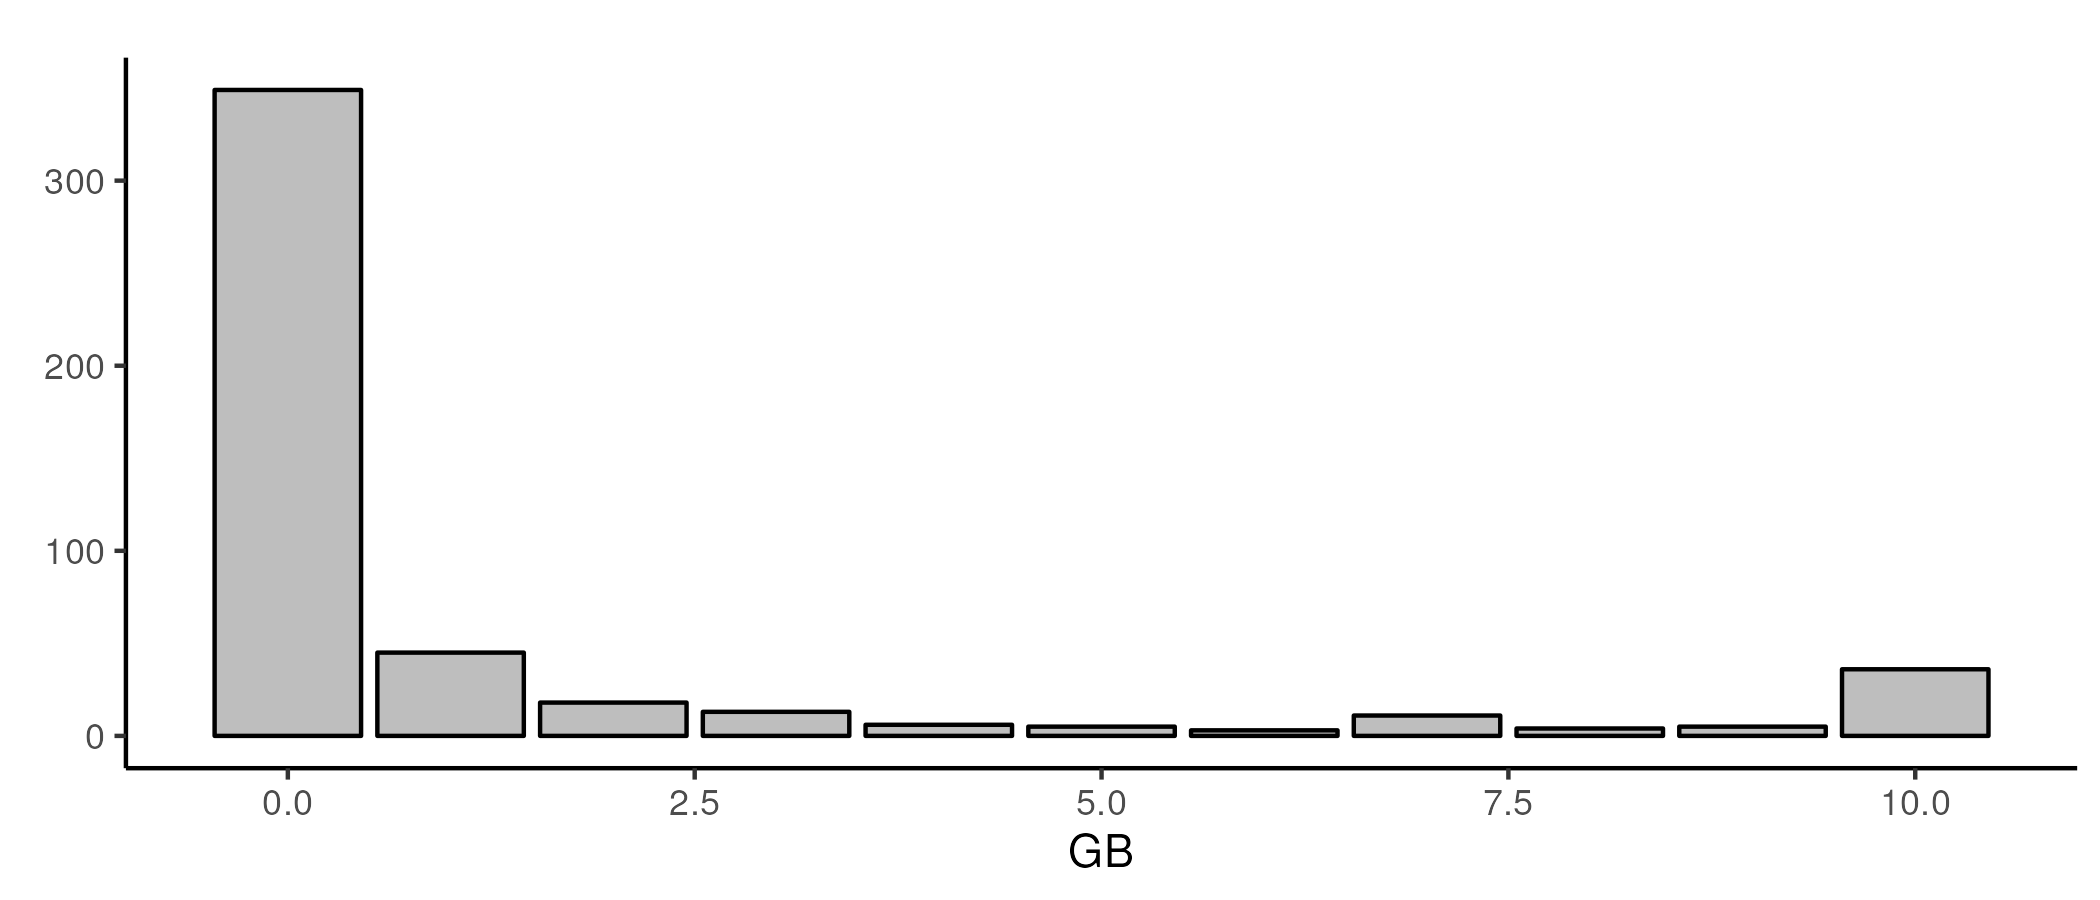
\includegraphics[width=\textwidth]{images/plot_filesize_dist.png} 
    \caption{Size distribution of replication packages deposited at openICPSR between  \firstday{} to \lastday{}, top-coded at 10GB.}
    \label{fig:size_packages}
\end{figure}


\subsection{Third-party repositories}

The \ac{DCAP} allows for code and data  to be deposited at other trusted repositories, as long as all other elements of the \ac{DCAP} are complied with. In fact, authors are \textit{discouraged} from duplicating deposits they have made elsewhere. This is intended to allow authors to create replication packages prior to submitting at the AEA's journals, or any other journal, as a component of a reproducible workflow and possibly in compliance with funder data management policies. Examples of other general purpose repositories include the \urlcite{https://dataverse.harvard.edu/}{Harvard Dataverse} and \purlcite{https://zenodo.org/}{Zenodo}. Authors depositing on Zenodo can request inclusion in the  ``AEA community'' at \href{https://zenodo.org/communities/aeajournals/}{zenodo.org/communities/aeajournals/}. For example, we work with authors to deposit  partial data packages on Zenodo when the size of the data files surpasses 30 GB. Some of these are deposited on Zenodo, where the  ``AEA community'' is available. Table~\ref{tab:webstats} shows a small number of very large packages on Zenodo, with \zenodototalSizeGB{}~GB of data  deposited in only \zenodototalPublished{} packages. 


More specific repositories that only allow specific authors to deposit (but anybody to obtain data from), such as the \purlcite{https://snd.gu.se/en}{Swedish National Data Service} or the new \curlcite{https://reproducibility.worldbank.org/}{World Bank Reproducible Research Repository} have been used more recently for partial or complete replication packages. In many of these cases, the Data Editor has actively assisted authors in preparing  data archives, and shared tools that make such data publication easier (see also next section).%
\footnote{Code to support uploading large quantities of data to Zenodo via the Zenodo API, originally created by LDI Lab Member Vansh Gupta, can be found at \href{https://github.com/AEADataEditor/Upload-to-Zenodo}{github.com/AEADataEditor/Upload-to-Zenodo}.}  Third-party repositories are linked to the main \aeadcr{} deposit, and are cited in the main article when appropriate. Authors wishing to deposit replication packages early in the research lifecycle are encouraged to consult the \curlcite{https://social-science-data-editors.github.io/}{Social Science Data Editors website} where links to trusted repositories are provided.  


\section{Providing Support for Compliance with AEA Data and Code Availability Policy}
\label{sec:dcap}

\subsection{Working with authors}

Since the introduction of the \ac{AEA}'s strengthened data and code availability policy in 2019 \citep{10.1257/pandp.110.dcap}, we have monitored how authors work to comply with the policy upon first submission of their packages. To help authors, we have published and continually update guidance available at  \href{https://aeadataeditor.github.io/}{aeadataeditor.github.io}. The  template README \citep{READMEv1.1.0}, which we published with several other economics data editors,  helps authors compile all the information required for complete documentation of their data and code deposit.\footnote{The README is available at \href{https://social-science-data-editors.github.io/template_README/}{social-science-data-editors.github.io/template\_README/}.} Guidance on specific topics is published in the form of blog posts.%
\footnote{Blog posts by the AEA Data Editor can be found at \href{https://aeadataeditor.github.io/year-archive/}{aeadataeditor.github.io/year-archive/}.}
%
%. Multiple presentations at workshops, conferences, and departmental seminars are also intended to clarify the AEA's policies on reproducibility, and convey best practices. Talks with materials are listed at \href{https://aeadataeditor.github.io/talks/}{aeadataeditor.github.io/talks/}. 
%In \reportyear{}, the Data Editor has given talks at the Banco de Portugal Workshop on Reproducibility, the Midwest Economics Association Meetings, a symposium on research transparency in Berlin, University of Virginia, the Meetings of the Western Economic Association, University of Tokyo, annual meeting of the Japanese Economic Association;  organized ``ask-me-anything'' sessions at the AEA Annual Meetings, UC Berkeley, Stanford, University of Toronto, Humbold University (Berlin); and organized (sometimes in conjunction with other data editors) tutorials and workshops at the European Economic Association, Universities of Tokyo and Osaka, and most recently at the 2024 AEA meetings.

% \subsection{Improving Findability of Replication Materials at the AEA}
% \label{sec:findability}

% We endeavor to make the replication packages provided by the authors broadly and easily findable. Naturally, they are linked from the article landing pages, but search engines  such as \urlcite{https://clarivate.com/webofsciencegroup/solutions/web-of-science/}{Web of Science} and \urlcite{https://scholar.google.com/}{Google Scholar} can also lead interested researchers to the replication packages directly. Authors are invited to fill out rich metadata as appropriate for their paper upon submission.\footnote{See guidance on metadata at \href{https://aeadataeditor.github.io/aea-de-guidance/data-deposit-aea.html}{aeadataeditor.github.io/aea-de-guidance/data-deposit-aea.html}.} 

% Authors are reminded that deposits receive their own \ac{DOI}, and should be cited in line with the Data Citation Principles \citep{Altman2013-fl,jddcp}. We continue to verify that authors cite all datasets they have used and accessed, as required by the AEA \ac{DCAP}, the AEA's citation requirements, and in line with the Data Citation Principles.  Data citations increase findability of data, allow data providers to receive proper credit, and align the Association with broader principles in the academic publishing world. The AEA's  \urlcite{https://www.aeaweb.org/journals/policies/sample-references}{Sample References} provide a style reference, and additional guidance for non-standard data sources, such as confidential or proprietary data, has been developed in collaboration with other journals and guidance by \purlcite{https://social-science-data-editors.github.io/guidance/addtl-data-citation-guidance.html}{librarians}



%\subsection{Compliance and Updates}
\label{sec:compliance}

We note that authors can be compliant with the policy without providing a copy of data used, as long as the reason for the inability to provide the data is acceptable, correct, and documented as part of the replication materials. 

Compliance with the policy %(Table~\ref{tab:compliance}) 
has been excellent. In some cases, we have requested data that was not initially provided, when such data could be legally and ethically provided; by the second round of assessments, compliance was generally achieved (see also our discussion of outreach to data providers).

Occasionally, a manuscript may be published while the replication package is still being updated. This leads to (temporary) non-compliance. Non-compliance may arise for technical reasons, such as when a file becomes corrupted in the upload process, preventing the deposit from being released. This year saw a week-long outage at ICPSR that lead to some temporary disruption in the processing of replication packages. In other instances, researchers have notified the Data Editor of a particular aspect of non-compliance - a file may be missing, a dataset may be able to be published that was not initially provided, etc. 
As of \lastday{}, \mcpubnoncompl{} packages were tagged as non-compliant.
%Column 1 in Table~\ref{tab:compliance} identifies the number of such cases as of \lastday{},  including deposits that have not yet been published. 
All cases are eventually resolved, either through pre-publication amendments, or post-publication updates.% (see next section).


% \begin{table}[t]
%     \centering
%     \caption{Compliance and Updates}
%     \label{tab:compliance}
    
%     \begin{threeparttable}
% %    \input{tables/n_compliance_manuscript}
%     \begin{tablenotes}
%     \footnotesize
%     \item[] \textit{Note}: Non-compliant deposits are a point-in-time estimate as of \lastday{} and do not reflect resolved non-compliance issues. Updates are unique submissions received regarding replication packages  between \firstday{} and \lastday{}. Updates are not counted in the overall count of assessments. 
%     \end{tablenotes}
%     \end{threeparttable}

%  \end{table}      
 


%\subsection{Post-publication modifications}

At the time of publication, a manuscript is linked with one (or more) archived replication packages, constituting the \textit{version of record} for the replication package. Occasionally, issues are brought to our attention by authors, readers, and data providers. Authors may have a better README, readers might have noticed a missing code or data file, or data providers might ask for a dataset to be removed because it infringes on terms of use agreed to by the author. The supplemental ``\textit{Policy on Revisions of Data and Code Deposits in the AEA Data and Code Repository}''\footnote{See Appendix~\ref{sec:list-of-policies} for a list of links to all supplemental policies.} specifies which modifications constitute a minor edit to the version of record, and which modifications lead to a higher version number, without modification of the existing version of record. In particular, any change that potentially changes a computational result or adds (untested) code will lead to a new version of the deposit being created, without changing or removing the version of record, even if the modifications fixes an error. However, the presence of replication packages that are newer than the version of record is signalled to readers via a banner, and is recorded in the metadata.

We identified \mcpubupdates{} actions regarding post-publication modifications in \reportyear{}.
%Column~2 in Table~\ref{tab:compliance} shows the distribution across journals. 
Table~\ref{tab:updates} identifies who initiated the updates.   Several updates were initiated following a  \textit{Replication Game} (see Section~\ref{sec:3rdparty} for details).

%\begin{table}[t]
%    \centering
\begin{center}
    \captionof{table}{Updates}{}
    \label{tab:updates}
    
     \begin{threeparttable}
     
% Table created by stargazer v.5.2 by Marek Hlavac, Harvard University. E-mail: hlavac at fas.harvard.edu
% Date and time: Wed, Dec 13, 2023 - 12:55:01 AM
\begin{tabular}{@{\extracolsep{5pt}} lc} 
\toprule 
Origin & Manuscripts \\ 
\midrule Author & 7 \\ 
Data Editor & 2 \\ 
Faculty & 2 \\ 
Other & 1 \\ 
Researcher & 4 \\ 
Student & 3 \\ 
\bottomrule 
\end{tabular} 

 
    \begin{tablenotes}
    \footnotesize
    \item[] \textit{Note}: Unit of observation are manuscripts assessed between \firstday{} and \lastday{}. A total of \mcpubupdates{} had updates; multiple origins of the information may have been identified.
    \end{tablenotes}
    \end{threeparttable}
\end{center}
%\end{table}

\subsection{Intellectual Property and Licenses} 
\label{sec:ip}

Authors retain  copyright for any data and code deposited by them in the \aeadcr{}, unless that copyright belongs to others and the authors have a license to republish it. The default license for all repositories based at openICPSR is the  Creative Commons Attribution (CC-BY) \citep{CreativeCommons2017}, but authors can choose their own license. All  licenses  are vetted by the Data Editor for compliance with the \ac{DCAP}. We encourage authors to consult our \purlcite{https://aeadataeditor.github.io/aea-de-guidance/licensing-guidance}{licensing guidance} 

In some cases, authors may wish to publish data under more restrictive licenses or conditions, due  mostly to ethical concerns, while ensuring that replication remains possible.%
\footnote{Examples from past years include \citet{deryugina2021data} and \citet{goncalves2021data}, which accompany \citet{deryugina_covid-19_2021} and \citet{goncalves_few_2021}, respectively.}
In the past, we have been able to leverage multiple mechanisms in place at the openICPSR repository hosting the \aeadcr{}; however, some of those mechanisms are no longer available. Authors who wish to explore ways to make their data ethically accessible should contact the Data Editor early enough in the submission process. 

The AEA replicators will sometimes access confidential or proprietary data for the purpose of verifying computational reproducibility (see Section~\ref{sec:verification}), as provided by the authors, or directly requested from the data providers via application or subscription services. Such data are not published as part of authors' replication packages. However, we do encourage authors to seek permission to share such data, where possible, and encourage data providers to allow for publication of extracts of their data, sufficient to support future reproducibility efforts. Table~\ref{tab:ndas} shows the number and type of agreements we entered into for the \mcpubnda{} formal or informal agreements in \reportyear{}.

\begin{minipage}{\columnwidth}
%\begin{table}[t]
%    \centering
\begin{center}
    \captionof{table}{NDAs and DUAs}{}
    \label{tab:ndas}
     \begin{threeparttable}
     
% Table created by stargazer v.5.2 by Marek Hlavac, Harvard University. E-mail: hlavac at fas.harvard.edu
% Date and time: Wed, Dec 13, 2023 - 12:55:01 AM
\begin{tabular}{@{\extracolsep{5pt}} lr} 
\toprule 
Type & Manuscripts \\ 
\midrule Data Use Agreement & 1 \\ 
NDA (formal) & 3 \\ 
NDA (informal) & 62 \\ 
\bottomrule 
\end{tabular} 

    \begin{tablenotes}
    \footnotesize
    \item[] \textit{Note}: Unit of observation are manuscripts assessed between \firstday{} and \lastday{}. 
    \end{tablenotes}
    \end{threeparttable}
\end{center}
\vspace{0.3cm}
%\end{table}
\end{minipage}

We continue to assist authors in remaining compliant with data use agreements and copyright law, to the extent possible, but authors should be aware of their potential liability in the cases of infringements. Since the summer of 2022, all authors are required to attest, via the published README, that they have ``\textit{legitimate access to and permission to use the data used}'' in the manuscript, and that they also have ``\textit{documented permission to redistribute [publish] the data}'' \citep[][pg.1]{READMEv1.1.0}. Unintentional posting of data that authors do not have permission to publish is one of the causes for replication packages being withdrawn, and thus becoming non-compliant until remediation and publication of an update.
%(thus showing up in Table~\ref{tab:compliance}).

\subsection{Direct outreach}

In order to reach authors and researchers with immediate or prospective questions, the Data Editor has presented and given workshops at McMaster University, Banco de Portugal, at  a Symposium on Open Science in Berlin, Université du Québec à Montréal, University of Tokyo, University of Osaka, and University of Virginia, as well as presentations or keynotes at the meetings of the Royal Economic Society, Midwest Economics Association, the Western Economic Association, the European Economic Association, and the Japanese Economic Association.
%
He also met with students and faculty  through informal in-person meetings and consultations at the ASSA meetings 2023, UC Berkeley, Stanford, University of Toronto, Humboldt University Berlin, and University of Tokyo.

\section{Working with Other Providers of Scientific Infrastructure to Improve Support for Documenting Provenance and Replicability}
\label{sec:coordination}

An important responsibility of the AEA Data Editor is to interact with other providers of scientific infrastructure. This includes other publishers and journals, archives such as ICPSR, providers of restricted or proprietary data, metadata harvesters, and third-party verification services. 


\subsection{AEA RCT Registry}
\label{sec:registry}

The \rctr{} (Registry) provides services to the economics (and social science) community at large. Managed at J-PAL and funded by the AEA, registration at the Registry is mandatory for field experiments published in \ac{AER}, \ac{AERI}, \ac{AEJAPP}, and \ac{AEJPOL}, but is also used more broadly in the economics discipline, with numerous publications in top economics journals as well as field journals identifying pre-registration in the Registry. The Registry is available at \href{https://www.socialscienceregistry.org/}{www.socialscienceregistry.org}.\footnote{This section is based in part on information provided by Stuti Goyal, Jack Cavanagh, and Sarah Kopper. All errors are mine.}
%
In collaboration with members of the AEA's \textit{Oversight Committee for Registry of Random Controlled Trials}, the Registry team at J-PAL have continued to work on improving the usability of the Registry, as well as ensuring the availability of Registry data. 


Data for the Registry is being curated and preserved in the \textit{AEA RCT Registry Dataverse} at 
\href{https://dataverse.harvard.edu/dataverse/aearegistry}{dataverse.harvard.edu/dataverse/aearegistry}, allowing for reproducible analysis of the universe of registrations by researchers.%
\footnote{Data shown in this report are derived from \citet{DVN/2RZF2X_2024}, and show data for calendar year \reportyear{}.  
%End-of-year numbers for \reportyear{} were extrapolated based on data from the first 11 months of \reportyear{}, as of \lastday{}. 
} 

% The Data Editor monitors proper reference to and citation of registrations. A registration should be cited in the text and the title footnote as, for example, ``\textit{Zhang (2017)}'' (the title footnote should also mention ``\textit{AEARCTR-0000005}''), and the references should have the appropriate entry:

% \begin{quote}\footnotesize
%     Zhang, Kelly. 2017. "Voter Pessimism and Electoral Accountability: Experimental Evidence from Kenya." AEA RCT Registry. May 02. https://doi.org/10.1257/rct.5-8.0.
% \end{quote}

%{\color{red}Additional data to come.}

%While the AEA journals mentioned above remain among the few economics journals that strictly require registration, 
Usage of the registration continues to increase strongly. As Figures~\ref{fig:registry1} and~\ref{fig:registry2} show, the rate of registrations per year continues to rise, and the registry now has over \regscumul{} registrations, which are being added at a rate of \regsyearly{} per year.  More than \registeredusers{} unique researchers are associated with these registrations (left panel, Figure~\ref{fig:registry2}), \activeusers{} of which are associated with registrations that have been active in \reportyear{}. The share of pre-registrations, favored by some, surpassed post-registrations for the first time in 2021, and remains higher (right panel, Figure~\ref{fig:registry2}). 

% src=https://github.com/J-PAL/AEA_registryanalysis/archive/refs/heads/main.zip

\begin{figure}
\centering
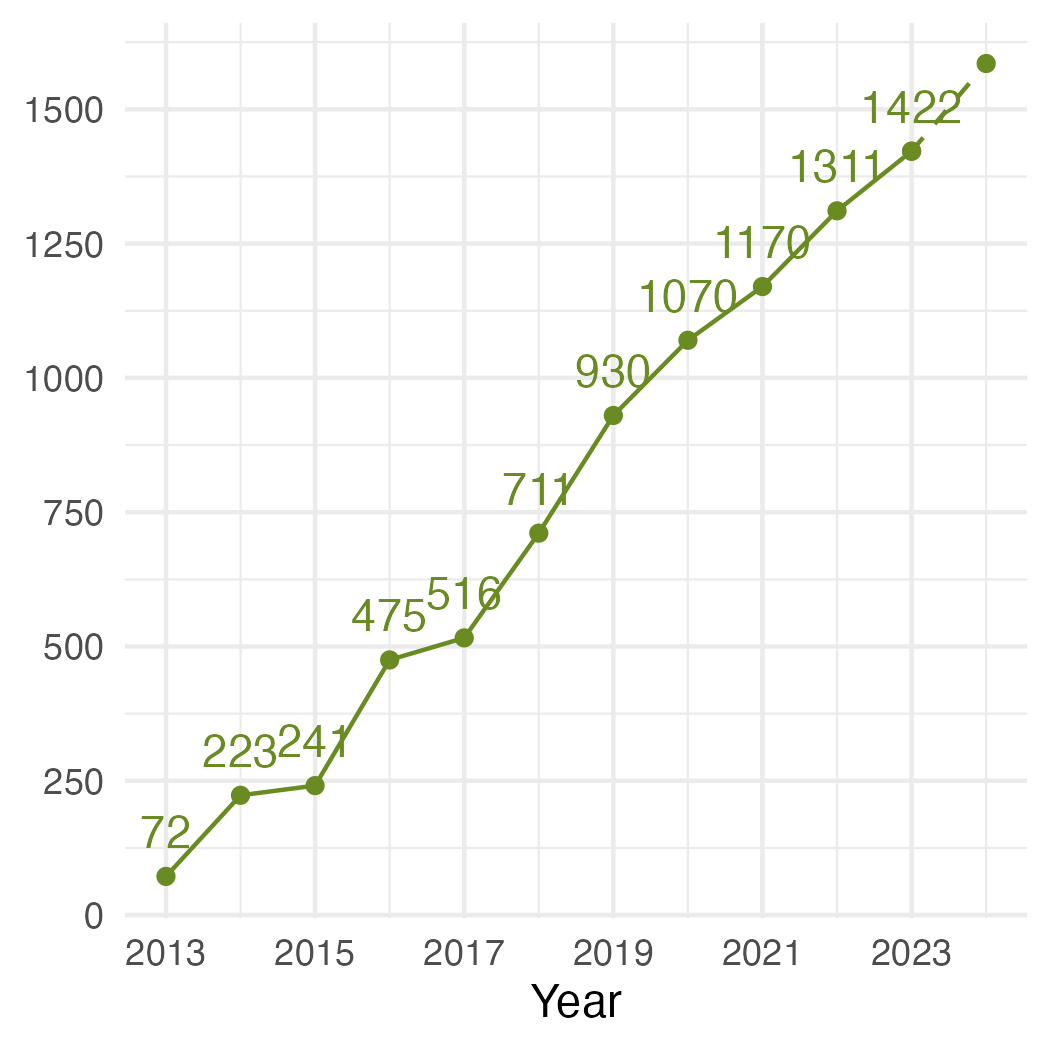
\includegraphics[width=0.4\textwidth]{data/registry/Output/reg_pre_year_2023.png}
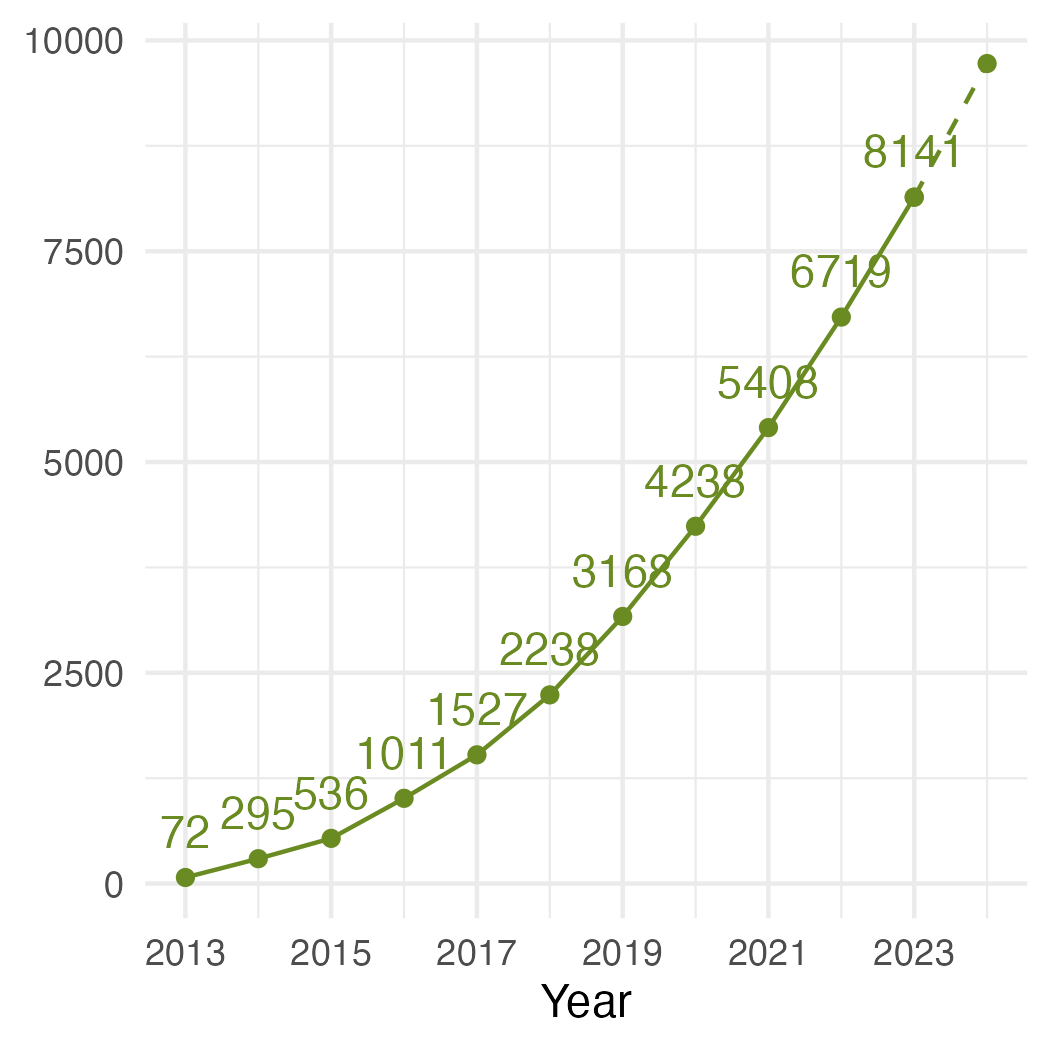
\includegraphics[width=0.4\textwidth]{data/registry/Output/reg_cumulative_2023.png}
\caption{Annual (left) and Cumulative Registrations (right) }
    \label{fig:registry1}
\caption*{\footnotesize Source: \citet{DVN/2RZF2X_2024}. Dashed lines are extrapolated increases for 2024.}
\end{figure}

\begin{figure}
\centering
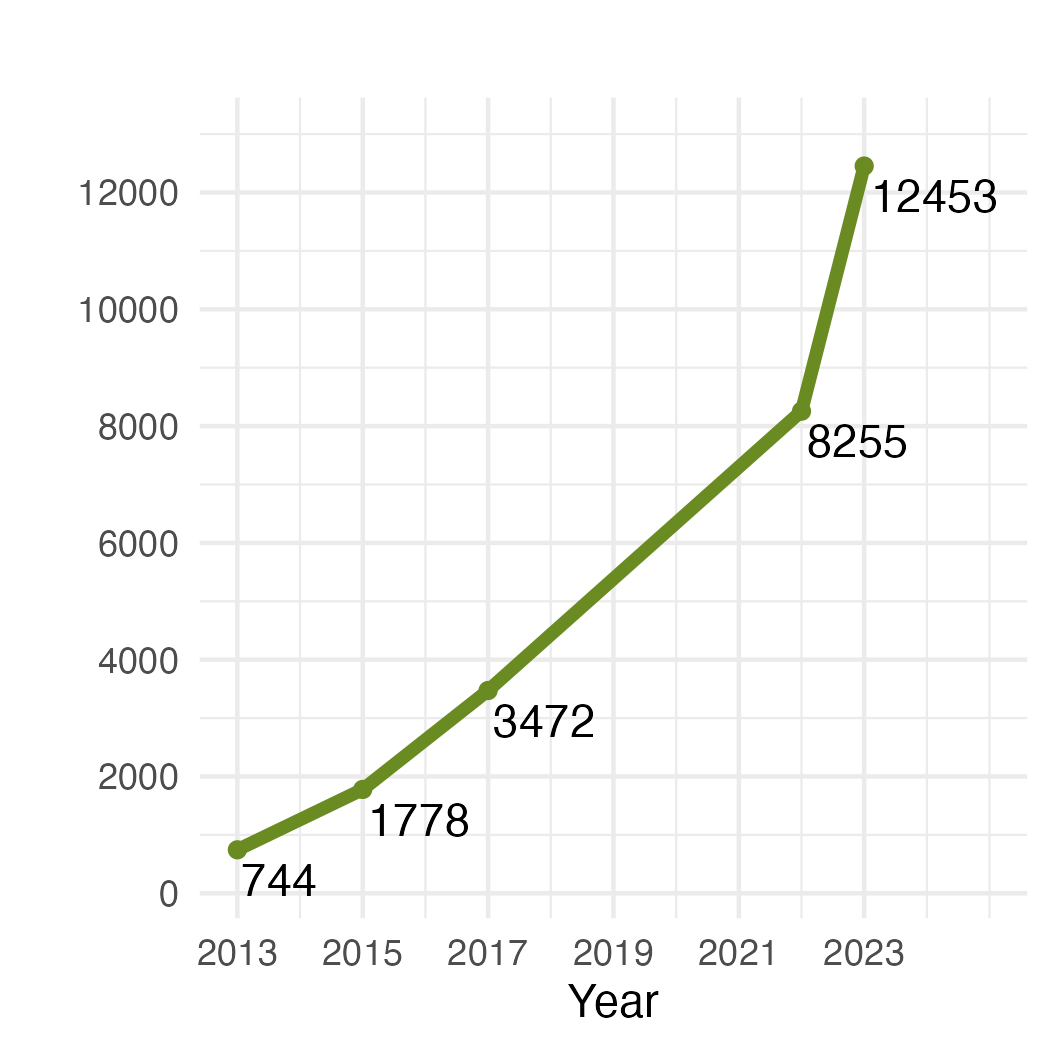
\includegraphics[width=0.4\textwidth]{data/registry/Output/registered_users_2023.png}
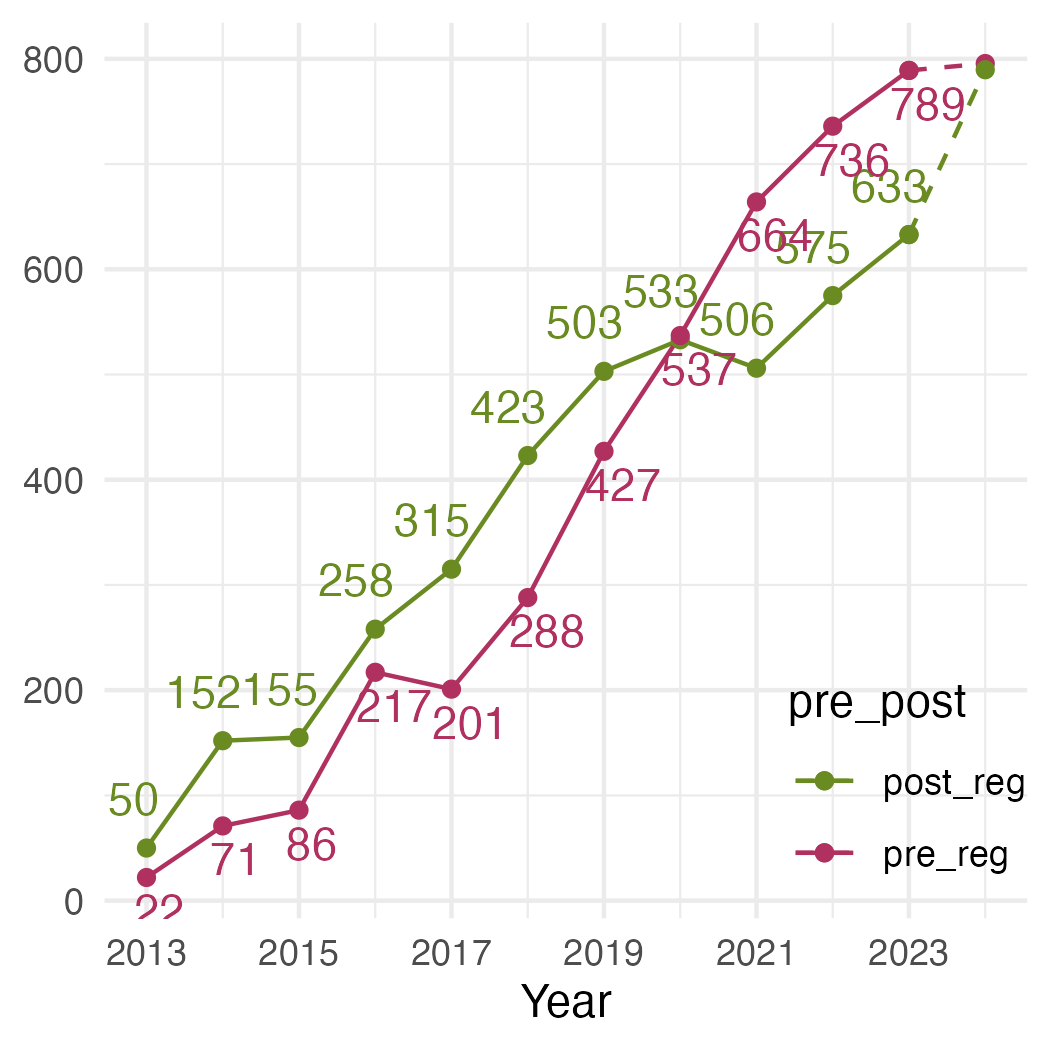
\includegraphics[width=0.4\textwidth]{data/registry/Output/post_pre_reg_2023.png}
\caption{Unique registered investigators (left), Post vs Pre-registrations (right)}
    \label{fig:registry2}
\caption*{\footnotesize Source: \citet{DVN/2RZF2X_2024}. Dashed lines are extrapolated increases for 2024.}
\end{figure}

As the registry has continued to grow, attract new users, and become a standard for experiments across economics and related social sciences, it is improving in its function as a central database of those experiments. In the last five years, an increasing number of articles  use the publicly available registry metadata as either their main analysis data or as a supplement to it. These can be grouped into a few broad sets.  
%
% In particular, multiple published articles and working papers use the Registry to analyze the scientific aspects of (pre-)registration, see \citet{corduneanu-huci_what_2022,
% miguel_evidence_2021,
% murtagh-white_learning_2023,
% leight_publication_2022,
% christensen_open_2019,
% ofosu_pre-analysis_2019,
% laitin_reporting_2021,
% abrams_research_2020,
% corduneanu-huci_politics_2021,
% buckley_role_2022,
% christensen_transparency_2018}.
%
%
One group of papers use the registry to study research transparency questions in the social sciences, either studying the registry as a transparency object in itself \citep{christensen_transparency_2018,abrams_research_2020,miguel_evidence_2021}, taking it as a means to glean information on other transparency behaviors \citep{ofosu_pre-analysis_2019,laitin_reporting_2021}, or  using it as an auditing tool, both for self-reported data \citep{christensen_open_2019} and the implementation of transparency policies \citep{buckley_role_2022}. A second group use the registry data as a significant portion of a larger compiled dataset attempting to proxy for the universe of experiments and experimenters in a particular subset of social science research \citep{corduneanu-huci_politics_2021,corduneanu-huci_what_2022}. A last group of studies use the data to answer meta-scientific questions about the studies on the registry \citep{leight_publication_2022,murtagh-white_learning_2023}.


% \subsection{Highlighting and Preserving Data Resources}

% We identified Zenodo as a possible solution to preserving large-scale data resources that surpass the practical capabilities of the \aeadcr{}. By creating the ``AEA Zenodo Community,'' we are able to highlight data resources that have, in the past, often not been curated or preserved appropriately. For instance, \citet{u_s_geological_survey_2022_5830968} comprises 83GB of data, preserved from DVDs and complemented and corrected manually based on online sources. They constitute some of the input data for \citet{10.1257/app.20200398}. Similarly, \citet{ministerio_de_desarrollo_productivo_arge_2022_6568295} preserves 44 GB of daily price data  captured in 2016-2018 and used by \citet{10.1257/mac.20210172}. In both cases, the data are under liberal licenses (public domain or Creative Commons licenses), which allow for the republication of the data. 


\subsection{Data Providers}
\label{sec:producers}

We regularly meet and communicate with academic, governmental, and commercial data providers, on behalf of specific authors or because we have identified a data provider as a frequently used resource. Discussion topics include making data citations easier, clarifying licenses, requesting blanket or streamlined data redistribution or access authorizations, or suggesting improved data curation practices to avoid repeatedly copying data from uncurated websites to the curated \aeadcr{}. 

In the course of the past year, we have talked about some or all of these topics with IPUMS, the World Bank (see also below), staff at the U.S. Census Bureau, the \ac{IRS}, the \ac{BLS}, the (German) Institute for Employment Research (IAB),  the \ac{BPLIM},  and the French \textit{Centre d'accès sécurisé de données} (CASD). We have also talked to various research groups on how to improve data curation, visibility, and citability of the data created by their efforts. 

\subsection{Economics Journals}

We continue to coordinate with other data editors conducting similar activities at other journals. An informal mailing list managed by the AEA Data Editor is used to interact with others.\footnote{Journal editors are encouraged to join the mailing list by contacting the AEA Data Editor.} Mailing list members who wish to be more actively involved can join the \textbf{monthly video call}, and participate in the development of the \purlcite{socialsciencedataeditors.github.io}{website of the Social Science Data Editors} In addition to the Data Editor of the AEA, the current group includes Miklós Koren (Data Editor, \acl{ReStud}), Florian Oswald (Data Editor, \acl{EJ} and Econometric Journal), Joan Llull (Data Editor, Econometrica),  Marie Connolly (Data Editor, \acl{CJE}), Anna Dreber Almenberg (Editor, JPE Microeconomics), and Maia G\"uell (Data Editor, \acl{JEEA}).  The website contains guidance on data citations and data availability statements, best practices for coding and data preparation, and links to various tools useful to replicators. In particular, the group coordinates the \textit{Template README} \citep{READMEv1.1.0}, which was last updated in November 2022, and which is referenced as a \textit{common} reference implementation for providing required information  across a number of journals. Furthermore, the group has developed a common standard for replication packages (\ac{DCAS}), which journals can use to signal that their requirements are similar to those commonly required by all endorsers of the standard \citep{datacodestandardv1}.%
\footnote{
After the 2024 Annual Meetings, but before final copy-editing for this report, the AEA's \acf{DCAP} was updated to conform to the order, format, and content of the \ac{DCAS}, see \href{https://www.aeaweb.org/journals/data/data-code-policy}{aeaweb.org/journals/data/data-code-policy}. The update does not change any requirements. The previous version of the policy can be found at \href{https://www.aeaweb.org/journals/data/archive/2020-2024}{aeaweb.org/journals/data/archive/2020-2024}. } 
%
Joint presentations and tutorials by the group involving the AEA Data Editor include the aforementioned presentations and workshops in Montréal (with Connolly), at the RES (with Connolly) and the EEA (with Koren).
%
The AEA Data Editor  also coordinates with the Editor and Data Editor of Economic Inquiry, and has had discussions with other editors and data editors seeking in put on their practices and policies. He furthermore participates in  the Steering Committee of a group of data repository leaders at Data-PASS organized as the Journal Editors Discussion Interface \purlcite{https://dpjedi.org/}{({JEDI})}


\subsection{Third-party verification services}
\label{sec:3rdparty}


We continue to rely on and have discussions with third-party verification services. As noted earlier, \jiraexternal{} reports were provided by external replicators or replication services
%for \jiramcsexternal{} manuscripts 
(see Table~\ref{tab:jirastats} for statistics by journal, and Appendix~\ref{app:3rdparty} for a list of third-party replicators). Of note, the World Bank has introduced a reproducibility \curlcite{https://reproducibility.worldbank.org/index.php/about}{verification service} which ``[verifies packages] to ensure that they are complete and fully functional before they are published to the repository.'' We will accept such third-party verifications, both at the time of submission as well as upon request, as long as the process by which they are created is documented and consistent with the approach that the economics journals are using. We are working on a mechanism to robustly  \purlcite{https://transparency-certified.github.io/}{``certify'' such processes}

\section{Working with the Economics Community to Enhance and Broaden Education on Replicable Science}

Outreach through presentations and publicly available tools is a key component of an effective data and code availability policy. 
%
Recordings of  presentations (when available) and presentation materials are listed at the \purlcite{https://aeadataeditor.github.io/talks/}{Data Editor's website} In addition to presentations, the Data Editor occasionally is an observer at \curlcite{https://i4replication.org/description.html}{Replication Games} where teams of researchers and students attempt to reproduce and extend papers published in leading economics journals. Such post-publication verifications are a necessary and useful check on published replication packages. Replicators may find issues that were not discovered, or discoverable, by pre-publication replicators such as the AEA Data Editor team. The Data Editor facilitates and monitors that any corrections or suggested improvements are conveyed to authors, and are reflected on replication packages via the AEA's \textit{Policy on Revisions of Data and Code Deposits} (see Appendix~\ref{sec:list-of-policies}). Several such (minor) corrections have lead to updates (see Table~\ref{tab:updates}). 
%


\subsection{Resources}

The AEA Data Editor maintains public resources available to the economics community. These are made available through a dedicated website at \href{https://aeadataeditor.github.io/}{aeadataeditor.github.io/} and code and project templates provided at \href{https://github.com/aeadataeditor}{github.com/aeadataeditor}. In particular:

\begin{itemize}
    \item Step-by-step guidance on how to prepare a replication package is provided at \href{https://aeadataeditor.github.io/aea-de-guidance/}{aeadataeditor.github.io/aea-de-guidance/}, including video tutorials and a description of the process. 
    \item The template README \citep{READMEv1.1.0} is referenced as part of the guidance, and separately accessible at \href{https://social-science-data-editors.github.io/template_README/}{social-science-data-editors.github.io/template\_README/}.
    \item Various blog posts on topics relating to computational reproducibility are posted at \href{https://aeadataeditor.github.io/year-archive/}{aeadataeditor.github.io/year-archive/}, and may be summarized on Twitter under the Data Editor's handle \href{https://twitter.com/AEAData}{@AEAData},  on Mastodon under \href{https://mstdn.social/@aeadata}{@aeadata@mstdn.social}, and on BlueSky under \href{https://bsky.app/profile/aeadata.bsky.social}{@aeadata.bsky.social}
    \item Instructions to replicators for assessing authors' replication packages are provided at \href{https://github.com/AEADataEditor/replication-template}{github.com/AEADataEditor/replication-template}.
    \item Template code for using containers for Stata, R, Julia, and Gurobi can be found by \href{https://github.com/AEADataEditor?q=docker&type=all&language=&sort=}{searching for ``docker`` on the Github site}.
    
\end{itemize}


\section{Replication team at Cornell University}

\subsection{Replicators} 
\label{app:replicators}

The following \textbf{\teamsize} students have provided excellent assistance in reproducing the results from the \jiramcs{} articles processed by the Replication Lab:
%
% Pulled from processing-jira...
%
%
Adam J. Faridi,
Akshay Yadava,
Alice Wei,
Amie Li,
Ananya Bakshi,
Andrew Phiri,
Andrew Wallace,
Anjini Khanna,
Anurag Tiwari,
Arnaav Sareen,
Bianca Jimenez,
Caitlin Song,
Crystal Lim,
Elian Gomez,
Ethan Carlson,
Gary Wu,
Hawi Tolera,
Ilona Khimey,
Jade Yang,
Jaeyoung Shim,
Jason Lan,
Jessica Rizzo,
Joshua Wallace,
Kareena Stowers,
Kate Chanpong,
Kayla Yang,
Kirin Eicher,
Kristine Li,
Leslie Geng,
Lincy Chen,
Luke Trautwein,
Manvir Chahal,
Melanie Brown,
Micere Mugweru,
Miranda Zhou,
Nguyen Vo,
Olivia Liu,
Phalguni Miraj,
Sherry Li,
Siddhi Malvankar,
Sohit Gurung,
Talia Boehm,
Tommy Wang,
Vidya Balaji,
Yuchang Tian.

%
Graduate students  Leonel Borja Plaza and Linda Wang and Research Aide Sofia Encarnación (all Cornell University) have been invaluable assistants in training and coordinating the work as well as developing the methods and procedures which we have made public.  Linda Wang contributed programming to this report. Sofia Encarnación contributed to all parts of the process. A description and evaluation of the training of replicators for the AEA's Data Editor team was published as \citet{vilhuber_teaching_2022}. The training and reference manual can be found at \purlcite{https://labordynamicsinstitute.github.io/ldilab-manual/}{online}

\subsection{Computing support}

We thank the Economics Department and the ILR School for providing us with computing resources at the Cornell Center for Social Sciences and the Bioinformatics cluster. 

\section{Third-party contributors}

\subsection{Replicators}
\label{app:3rdparty}

We are grateful to the  third-party replicators who assisted us with verifications when we were unable to access data or, in some cases, computing resources. 
%We do not name individuals when doing so would reveal information not already known to the manuscript's authors, naming the institution instead. Names are listed in no particular order.
%
Graduate research assistants at Stanford, Penn State University, and at Cornell helped us. We thank  Paulo Guimarães and staff at \ac{BPLIM} who contributed their  time to  run code  on confidential data and provide us with detailed knowledge about the data being used. We in particular want to again thank Olivier Akmansoy, Christophe Hurlin (Université d'Orléans), and Christophe Pérignon (HEC Paris), all of \href{https://cascad.tech}{cascad}, a certification agency for scientific code and data, who have been generous of their time and resources, and have provided us with multiple reports during this time.  

We do not name the authors with whom we signed non-disclosure agreements, or who otherwise provided us with access to data that could not be published. We are grateful for their flexibility and patience.

\subsection{Computing resources}
\label{app:3rdparty-computing}

We are grateful to Codeocean, NBER, WholeTale, and Harvard Business School, who all provided us with access to computing resources at no cost, and technical assistance when necessary. We use free academic resources on Github and Bitbucket. WholeTale is free to use for any academic user.


\section{Disclosures}
\label{sec:disclosure}

We received a generous compute and storage quota from \href{https://codeocean.com/}{Codeocean}, a free license to use Stata 17/18 for one year in cloud applications from \href{https://stata.com/}{Stata}, and a subaward on NSF grant \href{https://nsf.gov/awardsearch/showAward?AWD_ID=1541450&HistoricalAwards=false}{1541450} ``CC*DNI DIBBS: Merging Science and Cyberinfrastructure Pathways: The Whole Tale'' from the University of Illinois to evaluate the WholeTale platform for the purpose of reproducibility verification. None of the sponsors have reviewed this preliminary assessment, or have had influence on any of the conclusions of this document. Codeocean currently offers academic users a certain number of monthly free compute hours. WholeTale is free to use.


\section{Data and Code Availability Statement}
\label{sec:dcas}

All publicly available data and code used to generate figures and tables in this article are available \citep{report2023data,E117876V5}. Some detailed data from the editorial system, used for Table~\ref{tab:pre:rounds}, are considered confidential and cannot be made available in a way that preserves the privacy of the editorial process at this time.


\begin{flushright}
{\sc Lars Vilhuber}, \textit{Data Editor}
\end{flushright}


\FloatBarrier
% Remove or comment out the next two lines if you are not using bibtex.
%
% NOTE: Do not modify the AEADataEditor.bib manually!
%
\bibliographystyle{aea-mod}
\bibliography{paper,references,refs-zotero,registry-use}

% The appendix command is issued once, prior to all appendices, if any.
\appendix

\section{List of Policies}
\label{sec:list-of-policies}

All policies are listed at \url{https://www.aeaweb.org/journals/data}.

Main policy: \url{https://www.aeaweb.org/journals/data/data-code-policy}

Supplemental policies:
\begin{itemize}
    \item The \textit{ Policy for Papers Conducting Experiments and Collecting Primary Data} (\href{https://www.aeaweb.org/journals/data/policy-experimental}{aeaweb.org/journals/data/policy-experimental}) applies to laboratory experiments, field experiments, and any surveys, and specifies what should be provided in addition to the main policy.
    \item The \textit{Policy and Protocol for Third-Party Verifications} (\href{https://www.aeaweb.org/journals/data/policy-third-party}{aeaweb.org/journals/data/policy-third-party} specifies how we send out or accept verifications conducted by parties other than the Data Editor team.
    \item The \textit{Policy on Revisions of Data and Code Deposits in the AEA Data and Code Repository} (\href{https://www.aeaweb.org/journals/data/policy-revisions}{aeaweb.org/journals/data/policy-revisions}) applies when it becomes necessary to revise published replication packages. This may happen when readers and researchers contact the Data Editor, when authors identify a problem, correction, or improvement themselves, or when it becomes necessary for whatever reason to modify the replication package. The policy also defines under what conditions the version of record is modified, or whether the updated deposit simply becomes connected to, but does not replace the version of record.
\end{itemize}


\end{document}

